\documentclass[12pt]{beamer}
\usetheme{Boadilla}
\usepackage{graphicx}
\usepackage{algorithm2e}
\graphicspath{{images/}}
\title{CMPT 155: Computer Applications for Life Sciences}
\subtitle{Lecture 3: Navigating Through Excel Part 2}
\author{Ivan E. Perez}
\institute{}
\date{January 25, 2022}
\usepackage{booktabs} % Allows the use of \toprule, 
\usepackage{appendix}
\usepackage{enumerate,multicol}
\usepackage{amsmath, amssymb, amsthm}
\usepackage{tikz}

\begin{document}
	\begin{frame}
		\titlepage
	\end{frame}
	
	\begin{frame}
		\frametitle{Presentation Outline}
		\tableofcontents
		
	\end{frame}
	
\section{Selections}
	\begin{frame}
		\frametitle{Continuous Range Selection: Selecting Columns and Rows}
		To practice making selections we can:
		\begin{itemize}
			\item click and drag from cell you have selected
			\item select whole column by clicking on cell and pressing Ctrl + Shift + Down(Up)
			\item select whole row by clicking on cell and pressing Ctrl + Shift + Left(Right)
			\item select multiple adjacent columns/rows Hold Shift (Cmd) and drag.
		\end{itemize} 
	\begin{center}
		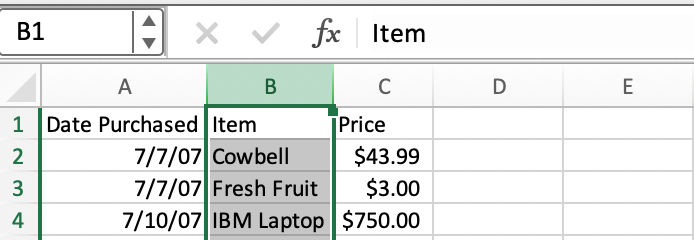
\includegraphics[width=0.5\textwidth]{continuous_selections.png}
	\end{center}
	\end{frame}
	
	\begin{frame}
		\frametitle{Discontinuous Selections}
		\begin{itemize}
			\item Discontinuous selections can be made by holding the Ctrl (Cmd) key. 
		\end{itemize}
	\begin{center}
		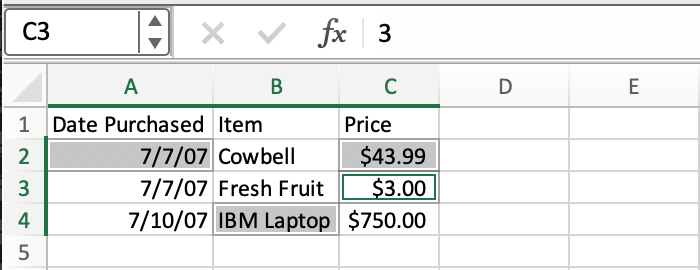
\includegraphics[width=0.5\textwidth]{discontinuous_selections.png}
	\end{center}
	\end{frame}

\section{Data Manipulation}

	\begin{frame}
		\frametitle{Cut-Paste or Copy-Paste}
		\begin{itemize}
			\item When you copy cells, everything comes along (text, numbers, formatting).
			\item Paste options
				\begin{itemize}
				\item Paste format (Ctrl + V) \item Paste value only
				\item Transpose
				\end{itemize}
		\end{itemize}
	\begin{figure}[htb]
		\begin{minipage}[t]{0.49\linewidth}\centering
			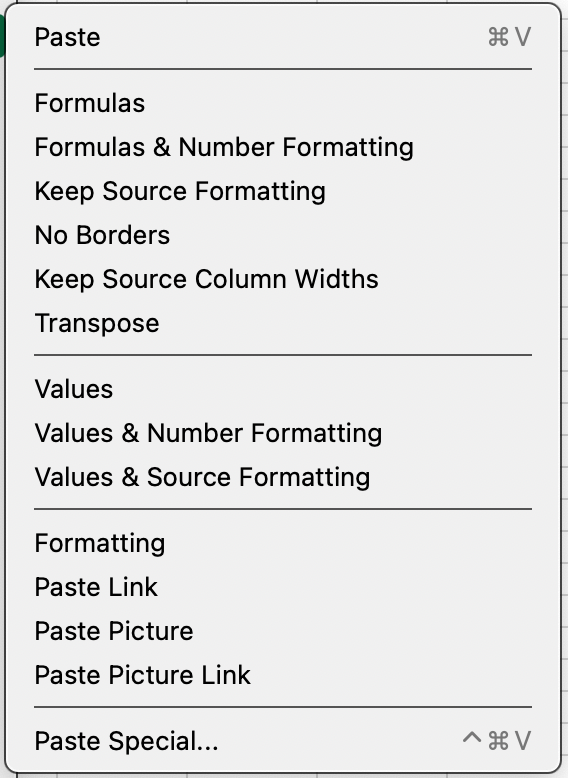
\includegraphics[width=0.49\linewidth]{pasteoptions.png}
			\medskip
			\centerline{(a)}
		\end{minipage}\hfill
		\begin{minipage}[t]{0.5\linewidth}\centering
			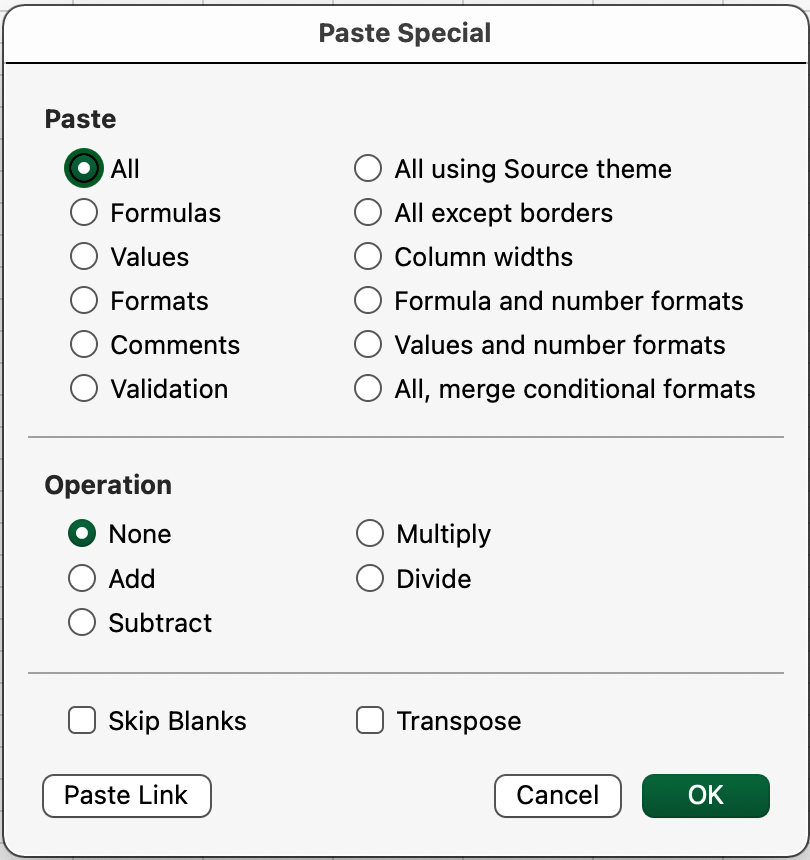
\includegraphics[width=0.5\linewidth]{pasteoptions_full.png}
			\medskip
			\centerline{(b)}
		\end{minipage}
	\end{figure}
		%\includegraphics[width=25mm]{Computer-$  $Applications-for-Life-Sciences.jpg}
	\end{frame}

	\begin{frame}
		\frametitle{Inserting Columns and Rows}
		\begin{itemize}
			\item Find the column immediately to the right of where you want to place the new column
			\item Find the row that is immediately below where you want to place the new row
		\end{itemize}
	\end{frame}
	
	\begin{frame}
		\frametitle{Deleting Columns and Rows}
		\begin{itemize}
			\item “Delete” clears the cell content, but does not remove the cells.
			\item Home $\rightarrow$ Cell $\rightarrow$ Delete
		\end{itemize}
	\end{frame}

	\begin{frame}
		\frametitle{Managing worksheets}
		\begin{itemize}
			\item Add and remove worksheets
			\item Name and Rearrange Worksheets
			\item  Move worksheets from one workbook to another
		\end{itemize}
	\begin{center}
		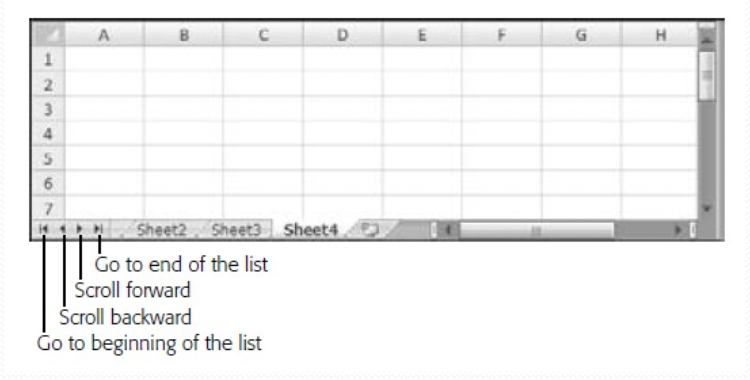
\includegraphics[width=0.5\textwidth]{managingworksheets.png}
	\end{center}
	\end{frame}

\section{Exercise}

	\begin{frame}
		\frametitle{Exercise}
		Download and modify the mailing list:
		\begin{enumerate}
			\item Copy the data in row 2, 3 and 4, paste them in row 5, 6
			and 7.
			\item Insert a column after the last name to store the ID information. Use AutoFill to fill the column. ID starts from 1001.
			\item Automatically adjust the columns to fit their content. \item Copy the mailing list and paste in transpose in Sheet2. 
			\item Adjust the column width of Sheet2.
			\item Rename Sheet1 and Sheet2.
			\item Save the workbook with a password.
		\end{enumerate}
	\end{frame}
\section{Find and Replace}
	\begin{frame}
		\frametitle{Find and Replace}
			\begin{itemize}
				\item Home $\rightarrow$ Editing $\rightarrow$ Find \& Select $\rightarrow$ Find (Ctrl + F)
				\item If you select a group of cells, Excel restricts the search to just those cells.
				\item Find All
				\item More Advanced Searches (Options)
				\item Home $\rightarrow$ Editing $\rightarrow$ Find \& Select $\rightarrow$ Replace (Ctrl + H)
				\item Hide the ribbon
			\end{itemize}
	\end{frame}

\end{document}





